
\subsection*{task 3.4 [10 points] \\[1ex] Hopfield nets: the $k$-rooks problem}

In lecture 10, we introduced the $k$-rooks problem and saw how to solve it using a Hopfield network. In particular, we considered the special case where $k=4$. Building on our discussion, here is what you are supposed to do in this task:

\begin{python}
# this is pretty much the exact code given in the lecture
# define the signum function
signum = lambda x: np.where(x >= 0, +1, -1)
# run the asynchronous hopfield network updates for some number of steps
def hopfield_run_async(s, W, theta, tmax=1000):
    for u in np.random.randint(0, s.shape[0], tmax):
        s[u] = signum(W[u, :] @ s - theta[u])
    return s
\end{python}
\begin{enumerate}
\item Use what we discussed in the lecture to implement a Hopfield net (with asynchronous updates) that solves the $k=4$ rooks problem; run your Hopfield net for, say, $100$ iterations

\begin{python}
# set the dimensions
k = 4
m = k * k
# build the hopfield network weight matrix
# as a block matrix consisting of J and I
I = np.eye(k)
J = np.full((k, k), 1.) - I
W = -0.5 * np.block([
    [J, I, I, I],
    [I, J, I, I],
    [I, I, J, I],
    [I, I, I, J]
])
# create the threshold vector
theta = np.full(m, (k - 2))
# create a random initial state
z = np.random.uniform(0, 1, size=m) >= 0.5
s = 2 * z - 2
# do a few hopfield state updates
s = hopfield_run_async(s, W, theta, tmax=100)
\end{python}

\item Now implement a Hopfield net that solves the $k=8$ rooks problem; to this end, you need to redefine or recompute the network parameters $\mat{W}_r$, $\mat{W}_c$, $\theta_r$, and $\theta_c$; the team with the ``most elegant'' numpy code to set these parameters will receive a honorary mention ;-)

\begin{python}
# set the dimension to 8 but the code fragment also
# works for arbitrary dimensions
k = 8
m = k * k
# 4-rooks problem
# build the weight matrix
# this works for arbitrary k
I = np.eye(k)
J = np.full((k, k), 1.) - I
W = -0.5 * np.block([
    [I] * i + [J] + [I] * (k - i - 1)
    for i in range(k)
])
# build the threshold vector
theta = np.full(m, (k - 2))
# create a random initial state
s = np.random.uniform(0, 1, size=m) >= 0.5
s = 2 * s - 1
# do a few hopfield state updates
s = hopfield_run_async(s, W, theta, tmax=100)
\end{python}

\item Run your Hopfield net for, say $100$ iterations and try to visualize the state it ends up in
\color{blue} \\[1ex]
\begin{figure}[hb]
    \centering
    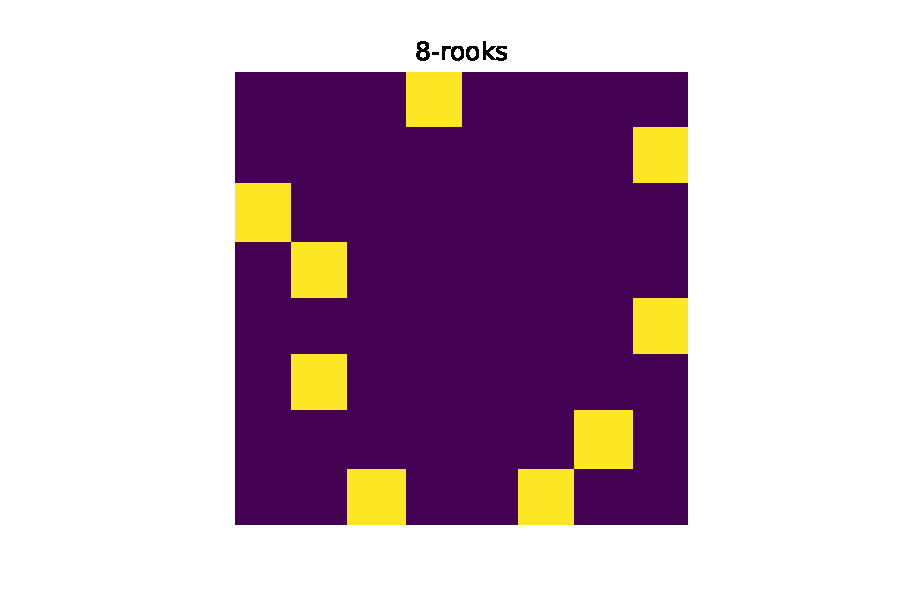
\includegraphics{Ex_03/Figures/8-rooks.pdf}
    \caption{Final state after 100 ansynchronus update steps.}
    \label{fig:my_label}
\end{figure}
\color{black}
\end{enumerate}



